\documentclass{snapshotmfo}
\categorizationmath{algebra and number theory,analysis,discrete mathematics and foundations,geometry and topology,numerics and scientific computing,probability theory and statistics} %at least one must be chosen. 
\categorizationconnect{chemistry and earth science,computer science,engineering and technology,finance,humanities and social sciences,life science,physics,reflections on mathematics} %can be void.
\license{CC-BY-SA-4.0} %recommended
\snapshotid{102}{1950}
\junioreditor{Some One}{junior-editors@mfo.de}
\senioreditor[f]{Carla Cederbaum}{senior-editor@mfo.de}
\director[m]{Gerhard Huisken}
\usepackage[utf8]{inputenc}
\usepackage{amsmath,amssymb}

\usepackage[ngerman]{babel}
%\usepackage[USenglish]{babel}

\author{Test Author}
\title{autoref with ngerman}
\begin{document}
\begin{abstract}
Check if the following autoref names are german:
\end{abstract}

\noindent \verb+\autoref{sec:heading}+ yields \autoref{sec:heading}.\\
\verb+\autoref{this}+ yields \autoref{this}.\\
\verb+\autoref{fig:sample-image}+ yields \autoref{fig:sample-image}.\\
\verb+\autoref{subsec:first}+ yields \autoref{subsec:first}.\\
\verb+\autoref{real}+ yields \autoref{real}.\\
\verb+\autoref{char.2}+ yields \autoref{char.2}.\\
\verb+\autoref{sec:another}+ yields \autoref{sec:another}.\\
\verb+\autoref{fig:maya}+ yields \autoref{fig:maya}.\\


\section{A heading}
\label{sec:heading}
This is a section.
Your actual snapshot.\footnote{This is a footnote.\label{this}}

\begin{figure}[ht]
        \centering 
        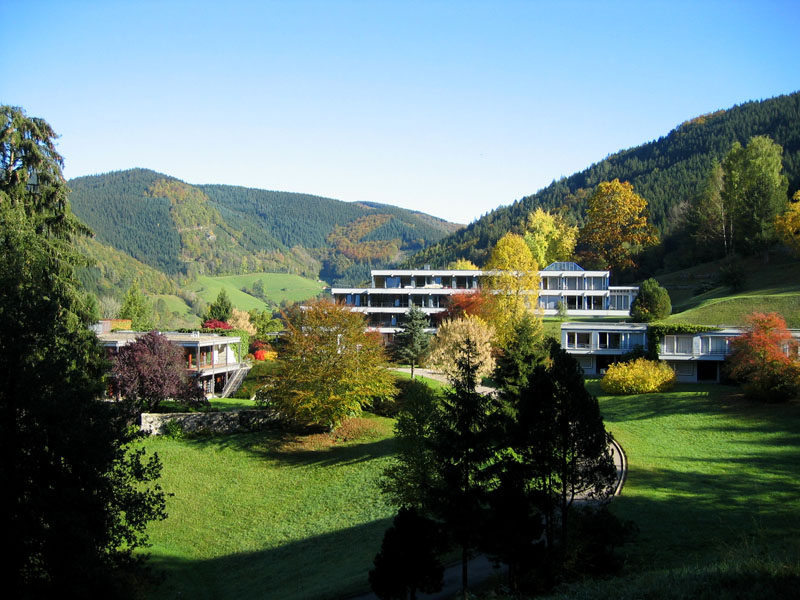
\includegraphics[width= 0.33 \textwidth]{mfo.jpg}
        \caption{An image scaled to 33\% of the textwidth.}
\label{fig:sample-image}
\end{figure}

\subsection{A subsection}
\label{subsec:first}
More text and some formulas:
\begin{align}\label{real}
1+1&=2,\\\label{char.2}
1+1&=0.
\end{align}
Formula \eqref{real} refers to $\mathbb{R}$, Formula \eqref{char.2} does not.


\section{Another section heading}
\label{sec:another}

\begin{figure}[ht]
        \centering 
        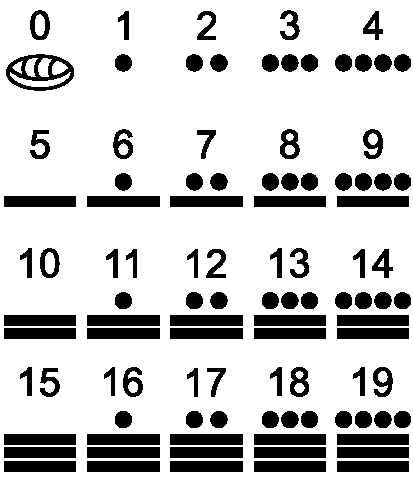
\includegraphics[width= 0.33 \textwidth]{maya.pdf}
        \caption{Exemplary image: Maya numerals.}
\label{fig:maya}
\end{figure}

\begin{imagecredits}
  \item[\autoref{fig:sample-image}] Archives of the Mathematisches Forschungsinstitut Oberwolfach,\\\url{http://www.mfo.de}, 2004.
  \item[\autoref{fig:maya}] ``Maya''. Author: Bryan Derkson. Licensed under Creative Commons Attribution-Share Alike 3.0 via Wikimedia Commons, \url{http://commons.wikimedia.org/wiki/File:Maya.svg}, visited on September 5, 2014.
\end{imagecredits}

\end{document}
